\section{Comparativo Final}

\begin{frame}{Custo por Iteração --- Todas as Abordagens}
    \begin{center}
        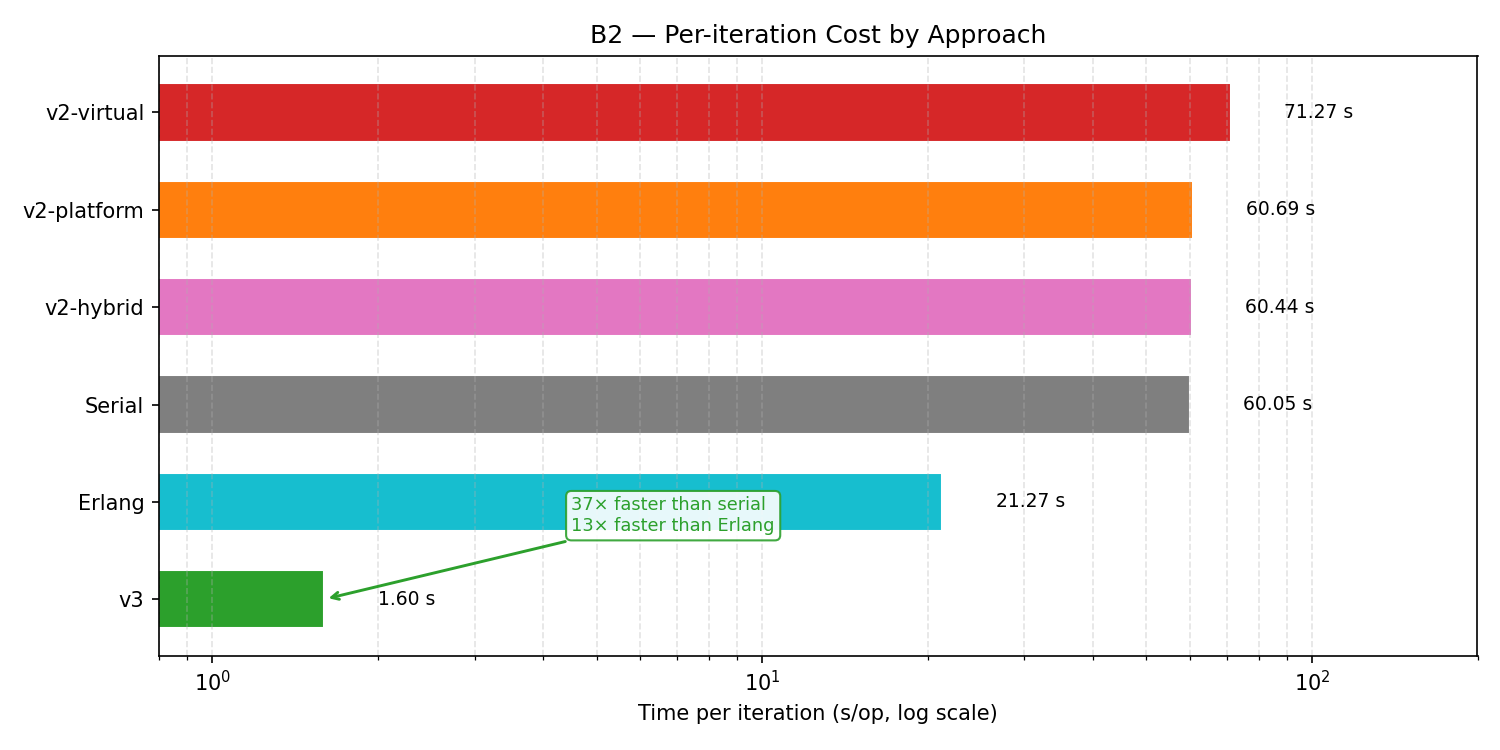
\includegraphics[width=0.90\textwidth]{img/chart1_b2_cost}
    \end{center}
\end{frame}

\begin{frame}{Evolução do Throughput}
    \begin{center}
        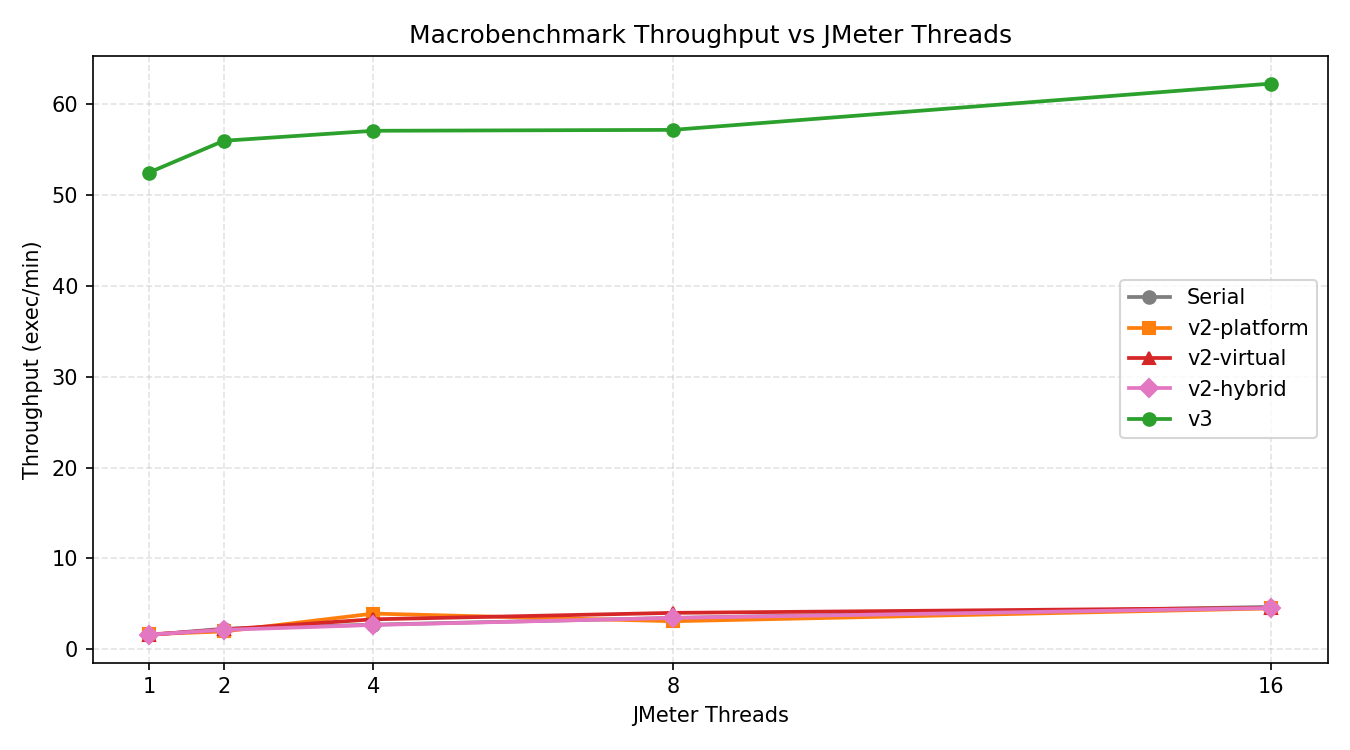
\includegraphics[width=0.90\textwidth]{img/chart2_macro_throughput}
    \end{center}
    {\small Painel superior: Serial e v2 (escala 0--7). Painel inferior: v3 (escala 0--70).}
\end{frame}

\begin{frame}{Trade-off: Releitura do CSV vs Dados em Memória}
    \begin{columns}
        \begin{column}{0.48\textwidth}
            \textbf{Releitura a cada iteração (v1/v2)}
            \begin{itemize}
                \item[\cmark] Baixo consumo de memória ($\approx$250 MB)
                \item[\cmark] Dataset pode ser maior que a RAM
                \item[\xmark] 82\% do CPU gasto em conversão de texto
                \item[\xmark] $\approx$12 s por iteração
            \end{itemize}
        \end{column}
        \begin{column}{0.48\textwidth}
            \textbf{Dataset em memória (v3)}
            \begin{itemize}
                \item[\cmark] Iterações 37$\times$ mais rápidas
                \item[\cmark] CPU dedicado 100\% ao algoritmo
                \item[\xmark] Heap de $\approx$2,7 GB necessário
                \item[\xmark] Dataset deve caber na RAM
            \end{itemize}
        \end{column}
    \end{columns}

    \vspace{0.5em}
    \begin{alertblock}{Lição}
        O JFR revelou onde o tempo realmente ia. Sem medir, paralelizaríamos
        os 8\% do algoritmo e ignoraríamos os 82\% do CSV.
    \end{alertblock}
\end{frame}

\begin{frame}{Quando Cada Modelo Vence}
    \begin{columns}
        \begin{column}{0.48\textwidth}
            \textbf{Java (memória compartilhada)}
            \begin{itemize}
                \item[\cmark] Aritmética 113--165$\times$ mais rápida
                \item[\cmark] Todos os núcleos ativos durante iteração
                \item[\cmark] Muito menos pressão de GC
                \item[$\cdot$] Ideal para cargas CPU-bound
            \end{itemize}
        \end{column}
        \begin{column}{0.48\textwidth}
            \textbf{Erlang (modelo de atores)}
            \begin{itemize}
                \item[\cmark] Race conditions impossíveis por construção
                \item[\cmark] GC sem pausas globais
                \item[\cmark] Escala para sistemas distribuídos
                \item[$\cdot$] Ideal para I/O intensivo e alta disponibilidade
            \end{itemize}
        \end{column}
    \end{columns}

    \vspace{0.5em}
    K-Means é CPU-bound com pouca comunicação entre iterações ---
    \alert{o caso em que memória compartilhada tem vantagem estrutural}.
\end{frame}
